\chapter{Work plan}\label{chap:chap4}

This chapter contains the methodology to be followed by the sequence of proposed tasks, with a brief description of the technologies and tools to be used in each phase of the development, and the global dissertation work planning.

\section{Methodology, Technologies and Tools}

The dissertation will be separated essentially in four phases. 

The first stage consists in a theoretical study and development of conceptual models that can be implemented to resolve the proposed problem. This will be supported and validated with functional simulations, using MATLAB or a similar tool. 

In a second phase of the project, the finalized mechanisms will be implemented in a CPU-FPGA platform, using Verilog Hardware Description Language and the XILINX Vivado design tool. Additionally, application software may be developed to facilitate the support and configuration of the system.

In the third and final stage, the field test will take place. First, it is intended to test the system in a confined underwater environment, such as the DEEC's tank. Then, the system will be tested in the ocean, as an outdoor realistic environment.

\section{Task timeline}

In this section it is proposed the work timeline for the second semester and the whole duration of the development of the dissertation research work. The intention is to complete the work topics as follows:

\begin{figure}[!htbp]
	\centering
	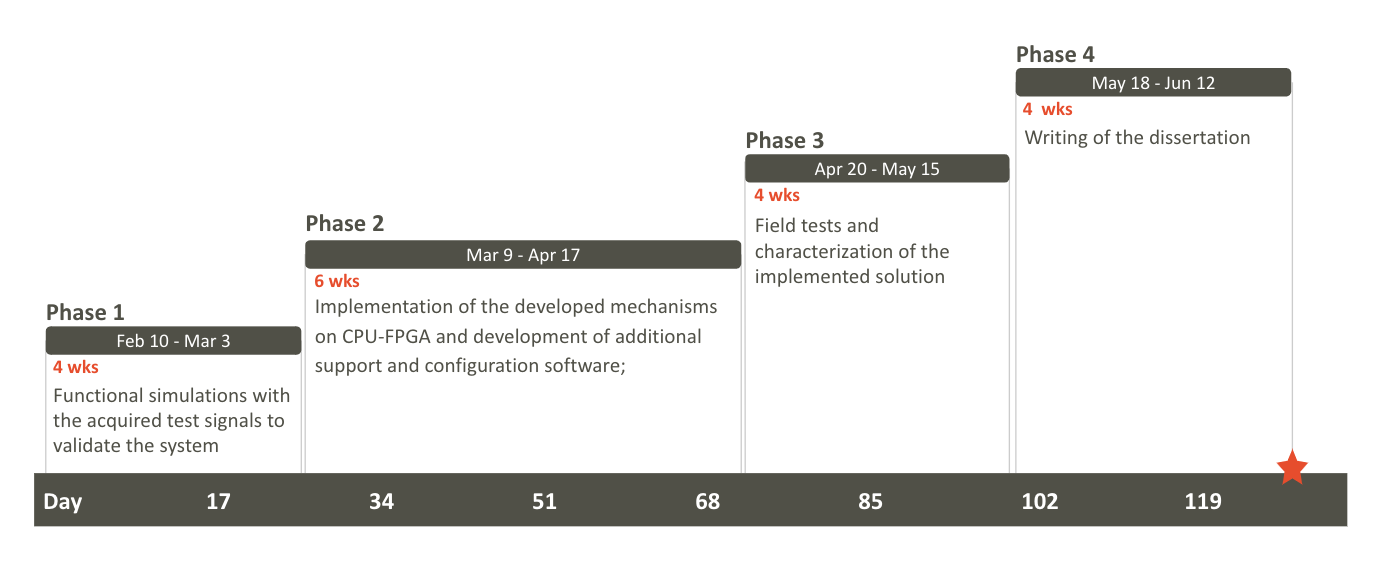
\includegraphics[width=1.1\textwidth]{figures/timeline}
	\caption{Work Plan Timeline}
	\label{fig:timeline}
\end{figure}

\begin{enumerate}
	\item \textbf{10/02 - 06/03 (4 weeks)} : Functional simulations (MATLAB or similar) with the acquired test signals to validate system;
	\item \textbf{09/03 - 17/04 (6 weeks)} : Implementation of the developed mechanisms on CPU-FPGA and development of additional support and configuration software;
	\item \textbf{20/04 - 15/05 (4 weeks)} : Field tests and characterization of the implemented solution;
	\item \textbf{18/05 - 12/06 (4 weeks)} : Writing of the dissertation.
	
\end{enumerate}
